% !Mode:: "TeX:UTF-8:Soft"
\ifx \allfiles \undefined
\documentclass[a4paper,12pt,twoside]{book}
\usepackage{CJKutf8}
\usepackage[T1]{fontenc}
\usepackage{pifont}
\usepackage{graphicx}
\usepackage{capt-of}
\usepackage{color}
\newcommand{\linuxcommand}[1]{\texttt{\textcolor{blue}{\$ #1 \Pisymbol{psy}{191}}}}
\newcommand{\op}[1]{\textcolor{blue}{-#1}}
\newcommand{\hotkey}[1]{\framebox{#1}}
\newenvironment{screen}{\sffamily}{\rmfamily}

\begin{document}
\begin{CJK*}{UTF8}{song}
\title{导言}
\author{赵岩}
\date{}\maketitle


\else
\chapter{Preface}
\fi
%上面的代码就是使得preface.tex也可以进行单独的编译。当然也可以被包含在book中进行编译。

Today, I have decided to make all my documents with the new tool --- \LaTeX.
\section*{Why I use Latex}
I have tried to record all my knowledge whenever and wherever, the previous tool is Microsoft Word. There are some problems, the first one is I can't run word in linux, so I can't update my word document in any computer. Another problem is the format of Word is BlackBox, It give you a lot of trouble when you write scienice document. A better solution is \LaTeX\ becuase it's nothing but a text file, you can update wherever you have text editor. And It can be changed to a good format with \LaTeX\ engine. \par

With help of ssh and svn, you can modify your document anyplace and anytime. Detail is listed in Figure  \ref{how-to-work}\\
\begin{center}
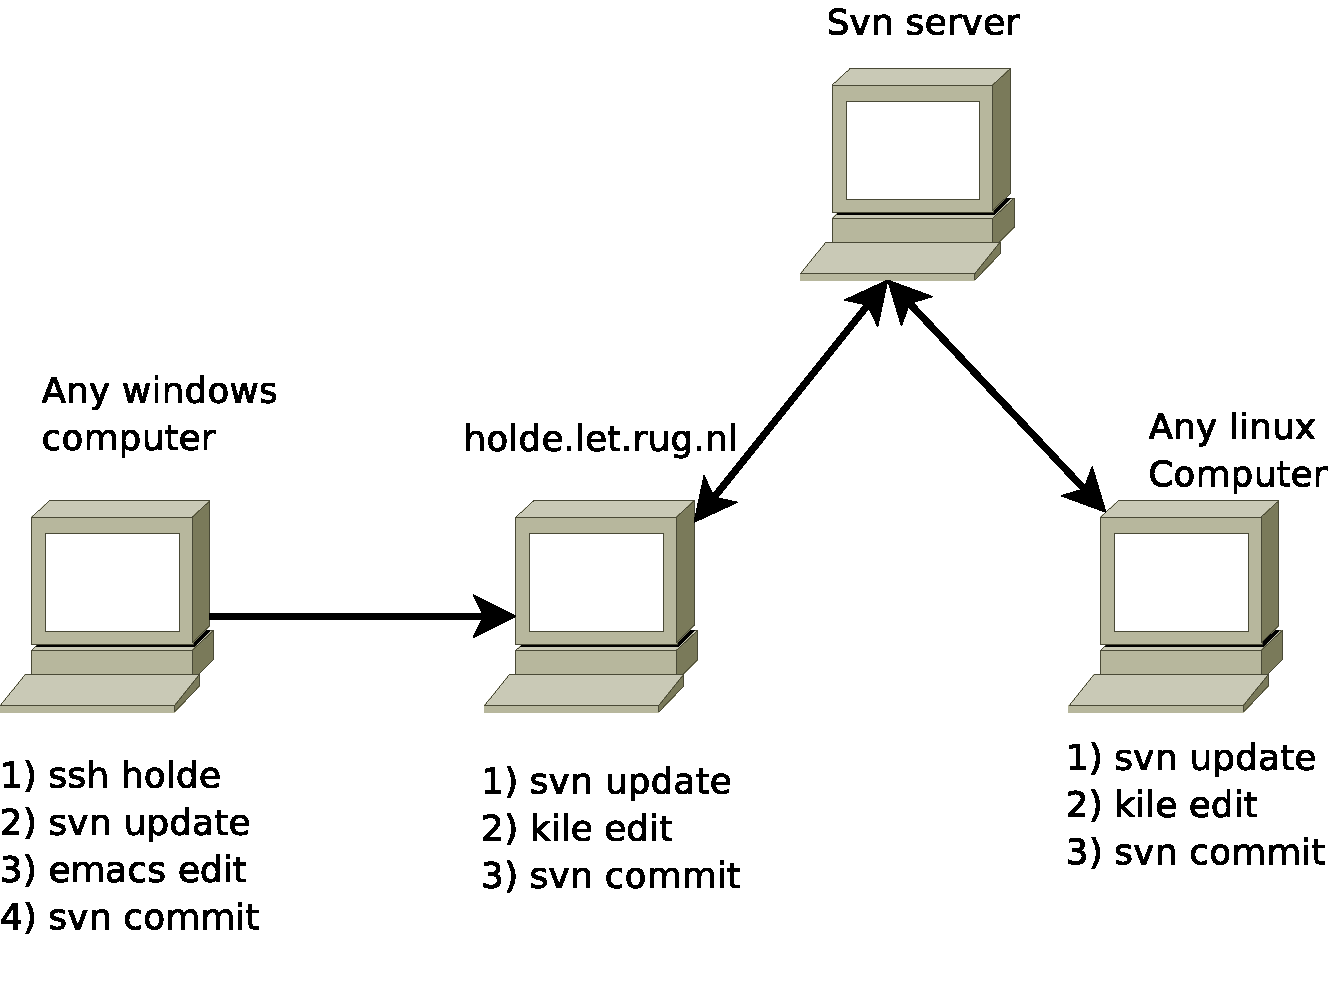
\includegraphics[scale=0.4]{pics/Doc_develop}
\captionof{figure}{How to work}
\label{how-to-work}
 % Doc_develop.eps: -11243639x-1 pixel, 300dpi, -95196.14x-0.01 cm, bb=0 0 639 481
\end{center}
\section*{Format of reading}
There is four kinds of format
	\begin{itemize}
	\item linux command looks like this: \linuxcommand{linux command}
	\item scree output looks like this:
	\begin{screen}
	 scree output
	\end{screen}
	\item options of command looks like: \op{option}
	\item hotkey looks like: \hotkey{hotkey}
	\item source code looks like:
	\begin{verbatim}
 		source code
	\end{verbatim}
	\end{itemize}

\ifx \allfiles \undefined
\end{CJK*}
\end{document}
\fi
